\documentclass[11pt,english,dvipsnames,aspectratio=169,handout]{beamer}\usepackage[]{graphicx}\usepackage[]{xcolor}
% maxwidth is the original width if it is less than linewidth
% otherwise use linewidth (to make sure the graphics do not exceed the margin)
\makeatletter
\def\maxwidth{ %
  \ifdim\Gin@nat@width>\linewidth
    \linewidth
  \else
    \Gin@nat@width
  \fi
}
\makeatother

\definecolor{fgcolor}{rgb}{0.345, 0.345, 0.345}
\newcommand{\hlnum}[1]{\textcolor[rgb]{0.686,0.059,0.569}{#1}}%
\newcommand{\hlstr}[1]{\textcolor[rgb]{0.192,0.494,0.8}{#1}}%
\newcommand{\hlcom}[1]{\textcolor[rgb]{0.678,0.584,0.686}{\textit{#1}}}%
\newcommand{\hlopt}[1]{\textcolor[rgb]{0,0,0}{#1}}%
\newcommand{\hlstd}[1]{\textcolor[rgb]{0.345,0.345,0.345}{#1}}%
\newcommand{\hlkwa}[1]{\textcolor[rgb]{0.161,0.373,0.58}{\textbf{#1}}}%
\newcommand{\hlkwb}[1]{\textcolor[rgb]{0.69,0.353,0.396}{#1}}%
\newcommand{\hlkwc}[1]{\textcolor[rgb]{0.333,0.667,0.333}{#1}}%
\newcommand{\hlkwd}[1]{\textcolor[rgb]{0.737,0.353,0.396}{\textbf{#1}}}%
\let\hlipl\hlkwb

\usepackage{framed}
\makeatletter
\newenvironment{kframe}{%
 \def\at@end@of@kframe{}%
 \ifinner\ifhmode%
  \def\at@end@of@kframe{\end{minipage}}%
  \begin{minipage}{\columnwidth}%
 \fi\fi%
 \def\FrameCommand##1{\hskip\@totalleftmargin \hskip-\fboxsep
 \colorbox{shadecolor}{##1}\hskip-\fboxsep
     % There is no \\@totalrightmargin, so:
     \hskip-\linewidth \hskip-\@totalleftmargin \hskip\columnwidth}%
 \MakeFramed {\advance\hsize-\width
   \@totalleftmargin\z@ \linewidth\hsize
   \@setminipage}}%
 {\par\unskip\endMakeFramed%
 \at@end@of@kframe}
\makeatother

\definecolor{shadecolor}{rgb}{.97, .97, .97}
\definecolor{messagecolor}{rgb}{0, 0, 0}
\definecolor{warningcolor}{rgb}{1, 0, 1}
\definecolor{errorcolor}{rgb}{1, 0, 0}
\newenvironment{knitrout}{}{} % an empty environment to be redefined in TeX

\usepackage{alltt}
\usepackage{fontspec}
\setsansfont[Mapping=tex-text]{Fira Sans}
\setcounter{secnumdepth}{4}
\setcounter{tocdepth}{4}
\usepackage[normalem]{ulem}
\usepackage[T1]{fontenc}
\usepackage{dcolumn}
\usepackage{booktabs}
\usepackage{bm}
\usepackage{setspace}
\makeatletter
\usetheme{metropolis}
\setbeamertemplate{frame footer}{Bosancianu | Schaub | Hertie School}
\setbeamerfont{page number in head/foot}{size=\tiny}
\setbeamercolor{footline}{fg=gray}
\usepackage{xcolor}
\setbeamercovered{dynamic}
\usepackage{tikz, tikz-cd, animate}
\usetikzlibrary{arrows, positioning, fit, shapes.misc, shapes, backgrounds, trees}
\usetikzlibrary{decorations.pathreplacing}
\usepackage{pgfplots}
\pgfplotsset{compat=1.10}
\usepgfplotslibrary{fillbetween}
\usepackage{pgfplotstable}
\usepackage[labelformat=empty]{caption}
% For table captions in Beamer
\usepackage[sectionbib]{apacite}
\renewcommand{\bibliographytypesize}{\footnotesize}
\makeatletter
\let\st@rtbibsection\@bibnewpage
\let\st@rtbibchapter\@bibnewpage
\makeatother
\usepackage{amsmath, mathtools}
\usepackage{xunicode}
\usepackage{hyperref}
\usepackage{pgfplots}
\makeatletter
\long\def\ifnodedefined#1#2#3{%
    \@ifundefined{pgf@sh@ns@#1}{#3}{#2}%
}
\pgfplotsset{
    discontinuous/.style={
    scatter,
    scatter/@pre marker code/.code={
        \ifnodedefined{marker}{
            \pgfpointdiff{\pgfpointanchor{marker}{center}}%
             {\pgfpoint{0}{0}}%
             \ifdim\pgf@y>0pt
                \tikzset{options/.style={mark=*}}
                \draw [densely dashed] (marker-|0,0) -- (0,0);
                \draw plot [mark=*,mark options={fill=white}] coordinates {(marker-|0,0)};
             \else
                \ifdim\pgf@y<0pt
                    \tikzset{options/.style={mark=*,fill=white}}
                    \draw [densely dashed] (marker-|0,0) -- (0,0);
                    \draw plot [mark=*] coordinates {(marker-|0,0)};
                \else
                    \tikzset{options/.style={mark=none}}
                \fi
             \fi
        }{
            \tikzset{options/.style={mark=none}}        
        }
        \coordinate (marker) at (0,0);
        \begin{scope}[options]
    },
    scatter/@post marker code/.code={\end{scope}}
    }
}
\makeatother
% Defines a checkmark
\def\checkmark{\tikz\fill[scale=0.4,color=orange](0,.35) -- (.25,0) -- (1,.7) -- (.25,.15) -- cycle;}
\newcommand{\indep}{\perp \!\!\!\! \perp}
\setbeamertemplate{itemize items}{\checkmark}
\usepackage{multirow}
\hypersetup{pdfauthor={Bosancianu and Schaub},
	pdftitle={Statistical Modeling and Causal Inference with R},
	pdfsubject={Week 11: Causal Mediation},
	pdfkeywords={Berlin, Hertie, 2020, week 11, RDD}}
\title{\textsc{Statistical Modeling and Causal Inference with R}}
\subtitle{Week 11: Causal Mediation}
\date{November 23, 2020}
\author{Manuel Bosancianu \hfill Max Schaub}
\institute{Hertie School of Governance}
\IfFileExists{upquote.sty}{\usepackage{upquote}}{}
\begin{document}
\maketitle

\begin{frame}
	\frametitle{Recap}
  
  \begin{columns}
		\begin{column}{0.3\textwidth}
			\begin{tikzpicture}[->,
			>=stealth',
			shorten >=1pt,
			auto,
			thick]
			
			\draw[fill=black, draw=black] (0,0) circle (0.5ex) node (a) [below, yshift=-0.2cm] {\large\texttt{D}};
			\draw[fill=black, draw=black] (2,0) circle (0.5ex) node (b) [below, yshift=-0.2cm] {\large\texttt{Y}};
			\draw[fill=black, draw=black] (1,-1.5) circle (0.5ex) node (c) [right, yshift=-0.2cm] {\large\texttt{H}};
			\draw[->, black] (0,0) -- (1.92,0);
			\draw[->, orange] (1,-1.4) -- (1,-0.01);
			\end{tikzpicture}
		\end{column}
		\begin{column}{0.7\textwidth}
			\footnotesize
			\textcolor{orange}{Moderation}: the magnitude of the ATE \textit{varies} systematically for sub-groups defined by \texttt{H}.\bigskip
			\pause
			
			 Example: effect of broadband availability on support for right-wing parties might be stronger for younger respondents \cite{schaub_voter_2020}.\bigskip
			 \pause
			
			In policy work, constitutes a check on whether specific groups are more exposed to benefits (or benefits) of intervention.
			
		\end{column}
	\end{columns}

\end{frame}




\begin{frame}
\frametitle{Interaction terms}

  \textcolor{orange}{Estimation}: done through multiplicative interaction terms \cite{brambor_understanding_2006}.
  
  \begin{equation}
    Y_i = \beta_0 + \beta_1D_i + \beta_2H_i + \beta_3D_i\times H_i + \epsilon_i
  \end{equation}\pause
  

\begin{itemize}
  \item $\beta_0$: intercept;
  \item $\beta_1$: effect of treatment on outcome, \textit{when} $H_i = 0$
  \item $\beta_2$: effect of mediator on outcome, \textit{when} $D_i = 0$ (control group)
  \item $\beta_3$: how effect of treatment changes for each unit change in $H_i$ (different subgroup)
\end{itemize}

\end{frame}


\begin{frame}
\frametitle{Graphical presentation}

\begin{figure}[!ht]
\centering
\begin{tikzpicture}[scale=0.9]
\begin{axis}[
	xlabel=Broadband availability, % label x axis
	ylabel=\% vote far-right, % label y axis
	axis lines=left, %set the position of the axes
	xmin=0, xmax=10, % set the min and max values of the x-axis
	ymin=1.7, ymax=2.0, % set the min and max values of the y-axis
	xticklabels={,,}, % Hide tick labels
	yticklabels={,,},
	clip=false
]

\draw [very thick] (0,66)--(80,186);
\draw [very thick, dashed] (0,66)--(80,16);
\draw [very thick] (0,86)--(80,36);
\draw [thick,->,>=stealth] (-1,66)--(-1,86) node [midway,left] {\scriptsize{$\beta_{older}$}};
\draw [thick,->,>=stealth] (40,126)--(60,126) node [midway,below] {\scriptsize{$1$}};
\draw [thick,->,>=stealth] (60,126)--(60,156) node [midway,right] {\scriptsize{$\beta_{BB}$}};
\node [fill=none] at (90, 6) {\scriptsize{Without $\times$}};
\node [fill=none] at (83, 46) {\scriptsize{$Old$}};
\node [fill=none] at (83, 196) {\scriptsize{$Young$}};
\draw[decorate,decoration={brace}, thick] (-1,0) -- node[left] {\scriptsize{$Intercept$}} (-1,66);
% Add the arrows for the interaction
\draw [thick,->,>=stealth] (20,96)--(20,73) node [midway,right, yshift=-2pt] {\tiny{$\beta_{*}$}};
\draw [thick,->,>=stealth] (40,126)--(40,61) node [midway,right, yshift=-11pt] {\scriptsize{$2\beta_{*}$}};
\end{axis}
\end{tikzpicture}
\caption{Example with broadband Internet (graph adapted from \citeNP{brambor_understanding_2006}). $\beta_{*}$ means $\beta_{older*BB}$.}
\end{figure}
\end{frame}


\begin{frame}
	\frametitle{Today's session}
	Identifying \textit{how} a treatment effect is transmitted:
	
	\begin{itemize}
	\setlength\itemsep{1.5em}
	  \item mediation in the classical LSEM tradition \cite{baron_moderator_1986}\pause
	  \item issues with the classical tradition \cite{bullock_mediation_2011}\pause
	  \item the \textit{causal mediation paradigm} \cite{imai_unpacking_2011}\pause
	  \item more practice with DAGs and the POF!
	  \item practical example with data from a job-seeking intervention
	\end{itemize}
	
\end{frame}


\begin{frame}
\frametitle{Today's example: JOBS II}
The JOBS II was a field experiment in Southeast Michigan in early 1990s.\bigskip

Treatment was a job-search skills seminar administered to unemployed persons. Control was a booklet with search tips.\bigskip
\pause

Expected effects:

\begin{itemize}
  \item increased employment\pause
  \item increased self-confidence $\Rightarrow$ decreased depression
\end{itemize}

\end{frame}


\begin{frame}
\frametitle{Today's example: JOBS II}

\begin{figure}
\begin{tikzpicture}[->,
			>=stealth',
			shorten >=1pt,
			auto,
			thick]
			
			\draw[fill=black, draw=black] (0,0) circle (0.5ex) node (a) [below, yshift=-0.2cm] {\large\texttt{Seminar}};
			\draw[fill=black, draw=black] (6,0) circle (0.5ex) node (b) [below, yshift=-0.2cm] {\large\texttt{Depression}};
			\draw[fill=black, draw=black] (3, 2.5) circle (0.5ex) node (c) [above] {\large\texttt{Confidence}};
			\draw[->, black] (0,0) -- (5.92,0);
			\draw[->, orange] (0.1,0.1) -- (2.93,2.44);
			\draw[->, orange] (3.13,2.44) -- (5.92,0.07);
			\end{tikzpicture}
\label{fig:01}
\end{figure}

How much of the \texttt{ATE} is \textit{transmitted} through improved self-confidence?

\end{frame}


\section{Classical mediation framework}

\begin{frame}
\frametitle{The Baron--Kenny model I}
Very influential across disciplines (to this day).

\begin{figure}
\begin{center}
    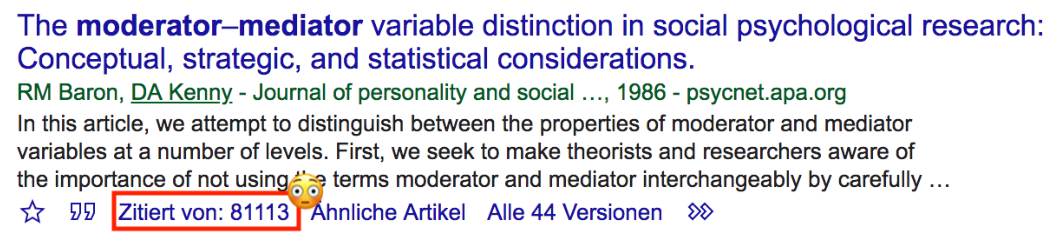
\includegraphics[scale=0.4]{../04-figures/11/01.PNG}
\end{center}
\label{fig:02}
\end{figure}

\begin{figure}
\begin{tikzpicture}
    \node[anchor=south west,inner sep=0] at (0,0) {
\includegraphics[scale=0.7]{../04-figures/11/02.PNG}};
    \draw[red,ultra thick] (1.1,0.1) rectangle (2.9,0.5);
\end{tikzpicture}
\end{figure}

\end{frame}


\begin{frame}
\frametitle{The Baron--Kenny model II}

\begin{columns}
		\begin{column}{0.5\textwidth}
\begin{figure}
\begin{tikzpicture}[->,
			>=stealth',
			shorten >=1pt,
			auto,
			thick,
			scale = 0.6]
			
			\draw[fill=black, draw=black] (0,0) circle (0.5ex) node (a) [below, yshift=-0.2cm] {\tiny{\texttt{Seminar}}};
			\draw[fill=black, draw=black] (6,0) circle (0.5ex) node (b) [below, yshift=-0.2cm] {\tiny{\texttt{Depression}}};
			\draw[fill=black, draw=black] (3, 2.5) circle (0.5ex) node (c) [above] {\tiny{\texttt{Confidence}}};
			\draw[->, black] (0,0) -- node[below] {a} ++(5.92,0);
			\draw[->, orange] (0.1,0.1) -- node[above,black] {b} ++(2.8,2.4);
			\draw[->, orange] (3.13,2.44) -- node[above,black] {c} (5.92,0.07);
			\end{tikzpicture}
\label{fig:03}
\end{figure}
\footnotesize

We also have a set of \textit{pre-treatment covariates}, \texttt{X}, which aren't included in the plot.
  \end{column}
  \pause
  \begin{column}{0.5\textwidth}
  \footnotesize
  
  $Seminar \Rightarrow Depression$: direct path ($a$ is the direct effect).\bigskip
  \pause
  
  $Seminar \Rightarrow Confidence \Rightarrow Depression$: indirect path, AKA ``front-door path'' (in POF).\bigskip
  \pause
  
  Indirect effect is a function of $b$ and $c$.
  
  \end{column}
\end{columns}

\end{frame}


\begin{frame}
  \frametitle{3 regressions}

   \footnotesize
   \begin{align}
   Depression_i &= \alpha_1 + \beta_1\overbrace{Seminar_i}^{treatment} + \zeta_1X_i + \epsilon_{i1} \label{eq:02}\\
   Confidence_i &= \alpha_2 + \beta_2Seminar_i + \zeta_2X_i + \epsilon_{i2} \label{eq:03}\\
   Depression_i &= \alpha_3 + \gamma Seminar_i + \beta_3\underbrace{Confidence_i}_{mediator} + \zeta_3X_i + \epsilon_{i3} \label{eq:04}
   \end{align}
  \pause
  \normalsize
  
  Total effect of $Seminar$ on $Depression$ is $\beta_1$ (Equation \ref{eq:02}).\bigskip
  
  To see how it's decomposed, substitute Equation \ref{eq:03} into Equation \ref{eq:04}.
  
\end{frame}


\begin{frame}
  \frametitle{Effect decomposition}
  \scriptsize
  \begin{align}
  Depression_i &= \alpha_3 + \gamma Seminar_i + \beta_3(\alpha_2 + \beta_2Seminar_i + \zeta_2X_i + \epsilon_{i2}) + \zeta_3X_i + \epsilon_{i3} \\
        &= \alpha_3 + \gamma Seminar_i + \beta_3\alpha_2 + \beta_3\beta_2Seminar_i + \beta_3\zeta_2X_i + \beta_3\epsilon_{i2} + \zeta_3X_i + \epsilon_{i3} \\
        &= \alpha_3 + Seminar_i(\gamma + \beta_3\beta_2) + X_i(\beta_3\zeta_2 + \zeta_3) + \beta_3(\alpha_2 + \epsilon_{i2}) + \epsilon_{i3}
  \end{align}
  \pause
  \normalsize
  
  $\beta_1$ (total effect) is now a composite term: $\gamma + \beta_2\beta_3$.\bigskip
  \pause
  
  $\gamma$ is the \textcolor{orange}{direct} effect of $Seminar$ on $Depression$.\bigskip
  
  $\beta_2\beta_3$ is the \textcolor{orange}{indirect} (or mediated) effect of $Seminar$ on $Depression$, transmitted through $Confidence$.
  
\end{frame}



\begin{frame}
  \frametitle{Configurations}
  
  \begin{columns}
  \begin{column}{0.32\textwidth}
  \footnotesize
  If $\gamma \approx 0$ and $\beta_2\beta_3 \neq 0$: full mediation.\bigskip
  
  \begin{figure}
  \begin{tikzpicture}[->,
			>=stealth',
			shorten >=1pt,
			auto,
			thick,
			scale = 0.4]
			
			\draw[fill=black, draw=black] (0,0) circle (0.5ex) node (a) [below, yshift=-0.2cm] {\tiny{\texttt{Seminar}}};
			\draw[fill=black, draw=black] (6,0) circle (0.5ex) node (b) [below, yshift=-0.2cm] {\tiny{\texttt{Depression}}};
			\draw[fill=black, draw=black] (3, 2.5) circle (0.5ex) node (c) [above] {\tiny{\texttt{Confidence}}};
			\draw[->, orange] (0.1,0.1) -- (2.92,2.43);
			\draw[->, orange] (3.13,2.44) -- (5.92,0.07);
			\end{tikzpicture}
	\end{figure}
  \end{column}
  \begin{column}{.01\textwidth}
  \rule{.2mm}{.8\textheight}
  \end{column}
  \begin{column}{0.32\textwidth}
  \footnotesize
  
  If $\gamma \neq 0$ and $\beta_2\beta_3 \approx 0$: no mediation.\bigskip
  
  \begin{figure}
  \begin{tikzpicture}[->,
			>=stealth',
			shorten >=1pt,
			auto,
			thick,
			scale = 0.4]
			
			\draw[fill=black, draw=black] (0,0) circle (0.5ex) node (a) [below, yshift=-0.2cm] {\tiny{\texttt{Seminar}}};
			\draw[fill=black, draw=black] (6,0) circle (0.5ex) node (b) [below, yshift=-0.2cm] {\tiny{\texttt{Depression}}};
			\draw[fill=black, draw=black] (3, 2.5) circle (0.5ex) node (c) [above] {\tiny{\texttt{Confidence}}};
			\draw[->, black] (0,0) -- (5.92,0);
			\end{tikzpicture}
	\end{figure}
  \end{column}
  
  \begin{column}{.01\textwidth}
  \rule{.2mm}{.8\textheight}
  \end{column}
  \begin{column}{0.32\textwidth}
  \footnotesize
  
  If $\gamma \neq 0$ and $\beta_2\beta_3 \neq 0$: partial mediation.\bigskip
  
  \begin{figure}
  \begin{tikzpicture}[->,
			>=stealth',
			shorten >=1pt,
			auto,
			thick,
			scale = 0.4]
			
			\draw[fill=black, draw=black] (0,0) circle (0.5ex) node (a) [below, yshift=-0.2cm] {\tiny{\texttt{Seminar}}};
			\draw[fill=black, draw=black] (6,0) circle (0.5ex) node (b) [below, yshift=-0.2cm] {\tiny{\texttt{Depression}}};
			\draw[fill=black, draw=black] (3, 2.5) circle (0.5ex) node (c) [above] {\tiny{\texttt{Confidence}}};
			\draw[->, black] (0,0) -- (5.92,0);
			\draw[->, orange] (0.1,0.1) -- (2.93,2.44);
			\draw[->, orange] (3.13,2.44) -- (5.92,0.07);
			\end{tikzpicture}
	\end{figure}
  \end{column}
  
  \end{columns}
  
\end{frame}


\begin{frame}
  \frametitle{JOBS II data}
  Outcome: continuous, score on Hopkins Symptom Checklist, measured 6 months after treatment.\bigskip
  
  Mediator: job search self-efficacy, measured 2 months after treatment.\bigskip
  \pause
  
  Covariates: age, education, gender, ethnic minority, depression measured during treatment, economic hardship, marital status, occupation, income.
  \pause
  

  
 \footnotesize
   \begin{align}
   Depression_i &= \alpha_1 + \beta_1\overbrace{Seminar_i}^{treatment} + \zeta_1X_i + \epsilon_{i1} \\
   Confidence_i &= \alpha_2 + \beta_2Seminar_i + \zeta_2X_i + \epsilon_{i2}\\
   Depression_i &= \alpha_3 + \gamma Seminar_i + \beta_3\underbrace{Confidence_i}_{mediator} + \zeta_3X_i + \epsilon_{i3}
   \end{align}
  
\end{frame}


\begin{frame}
  \frametitle{Results}
  




\begin{table}
\caption{Results from 3 specifications}
\begin{center}
\begin{footnotesize}
\begin{tabular}{l D{.}{.}{4.6} D{.}{.}{4.6} D{.}{.}{4.6}}
\toprule
 & \multicolumn{1}{c}{DV: Depression} & \multicolumn{1}{c}{DV: Confidence} & \multicolumn{1}{c}{DV: Depression} \\
\midrule
(Intercept) & 0.895^{***} & 3.870^{***} & 1.499^{***}  \\
            & (0.133)     & (0.159)     & (0.158)      \\
Seminar     & -0.047      & 0.101^{*}   & -0.032       \\
            & (0.035)     & (0.042)     & (0.035)      \\
Confidence  &             &             & -0.156^{***} \\
            &             &             & (0.023)      \\
\midrule
R$^2$       & 0.244       & 0.116       & 0.271        \\
Adj. R$^2$  & 0.230       & 0.100       & 0.256        \\
Num. obs.   & 1285        & 1285        & 1285         \\
\bottomrule
\multicolumn{4}{p{9.5cm}}{\tiny{$^{***}p<0.001$; $^{**}p<0.01$; $^{*}p<0.05$. Estimates from pre-treatment covariates have been excluded from the table.}}
\end{tabular}
\end{footnotesize}
\label{tab:01}
\end{center}
\end{table}

At this point, the manual calculations begin\dots
  
\end{frame}


\begin{frame}
\frametitle{Computing effects}

\begin{itemize}
\setlength\itemsep{1.5em}
  \item Direct effect: -0.032\pause
  \item Indirect effect: $\beta_2\times \beta_3$ = $0.101\times -0.156$ = -0.016\pause
  \item Total effect: $direct + indirect$ = $-0.032 + (-0.016)$ = $-0.047$ (rounding)
\end{itemize}
\pause

Aside from point estimates, we also need estimates of uncertainty:

\begin{itemize}
  \item $Seminar \Rightarrow Confidence$ = $b$
  \item $Confidence \Rightarrow Depression$ = $c$
\end{itemize}

\end{frame}


\begin{frame}
\frametitle{Computing uncertainty}

\begin{equation}
  SE_{indirect} = \sqrt{c^2\sigma_b^2 + b^2\sigma_c^2 + \sigma_b^2\sigma_c^2}
\end{equation}




\begin{table}
\footnotesize
\begin{tabular}{l D{.}{.}{4.6} D{.}{.}{4.6}}
\toprule
  & \multicolumn{1}{c}{Direct} & \multicolumn{1}{c}{Indirect} \\
\midrule
$\beta$ & -0.032 & -0.016^{*} \\
SE  &  (0.035) & (0.007) \\ 
\bottomrule
\end{tabular}
\end{table}
\pause

A case of pure mediation: a negative indirect effect of seminar attendance on depression (via confidence).

\end{frame}


\section{Challenges in classical framework}

\begin{frame}
\frametitle{Cracks in the foundation}
The approach established itself as \textit{de facto} standard in social and political psychology, and connected fields.\bigskip
\pause

Problems:

\begin{itemize}
\setlength\itemsep{1.5em}
  \item bias in OLS estimates\pause
  \item inability to cope with more complex causal structures\pause
  \item mostly obscures identification assumptions\pause
  \item does not extend to nonlinear models
\end{itemize}

\end{frame}

\begin{frame}
\frametitle{Bias in estimates}
 \footnotesize
   \begin{align}
   Depression_i &= \alpha_1 + \beta_1Seminar_i + \zeta_1X_i + \epsilon_{i1} \\
   Confidence_i &= \alpha_2 + \beta_2Seminar_i + \zeta_2X_i + \epsilon_{i2}\\
   Depression_i &= \alpha_3 + \gamma Seminar_i + \beta_3Confidence_i + \zeta_3X_i + \epsilon_{i3}\label{eq:05}
   \end{align}
   \normalsize
   
   In Equation \ref{eq:05}, $\beta_3$ is potentially estimated with bias:
   
   \begin{equation}
     \hat{\beta}_3 = \beta_3 + \frac{cov(\epsilon_{i2}, \epsilon_{i3})}{var(\epsilon_{i2})}
   \end{equation}\pause
  
  The only way $\hat{\beta}_3 = \beta_3$ and $\hat{\gamma} = \gamma$ is if $cov(\epsilon_{i2}, \epsilon_{i3}) = 0$.
  \pause
  
  This only holds if treatment and mediator are randomly assigned---not the typical design setup!

\end{frame}


\begin{frame}
\frametitle{Complex causal structures + obscuring identification}
 
\begin{columns}
	\begin{column}{0.45\textwidth}
		\begin{figure}
			\begin{tikzpicture}[->,
				>=stealth',
				shorten >=1pt,
				auto,
				thick,
				scale = 0.6]
				
				\draw[fill=black, draw=black] (0,0) circle (0.5ex) node (a) [below, yshift=-0.2cm] {\texttt{D}};
				\draw[fill=black, draw=black] (6,0) circle (0.5ex) node (b) [below, yshift=-0.2cm] {\texttt{Y}};
				\draw[fill=black, draw=black] (3, 2.5) circle (0.5ex) node (c) [above] {\texttt{M}};
				\draw[fill=black, draw=black] (3, -2.5) circle (0.5ex) node (d) [below] {\texttt{N}};
				\draw[->, black] (0,0) -- (5.92,0);
				\draw[->, black] (0.1,0.1) -- (2.92,2.46);
				\draw[->, black] (3.13,2.44) -- (5.92,0.07);
				\draw[->, black, dashed] (0.1,-0.1) -- (2.92,-2.46);
				\draw[->, black, dashed] (3.13,-2.44) -- (5.92,-0.07);
				\draw[->, orange, dashed] (3,-2.45) -- (3,2.47);
			\end{tikzpicture}
			\label{fig:04}
		\end{figure}
		\footnotesize
		\bigskip
		
		\texttt{N} is another causal pathway from treatment (\texttt{D}) to outcome (\texttt{Y}).
	\end{column}
	\pause
	\begin{column}{0.55\textwidth}
		\footnotesize
		Even with \texttt{D} and \texttt{M} randomized, $cov(\epsilon_{i2}, \epsilon_{i3}) \neq 0$ if \texttt{N} is unobserved.\bigskip
		\pause
		
		``Multiple-mediator'' problem: this can still bias estimates (and poses measurement challenges).\bigskip
		\pause
		
		Even when measuring all, ``one-at-a-time'' estimation of indirect effects is very likely inducing bias: omitted variables.\bigskip
		\pause
		
		Focus is on model fit and required covariates, rather than highlighting assumptions needed for identification.
		
	\end{column}
\end{columns}

\end{frame}


\begin{frame}
	\frametitle{Problem with nonlinearity}
	
	\begin{columns}
		\begin{column}{0.45\textwidth}
			\begin{figure}
				\begin{tikzpicture}[->,
					>=stealth',
					shorten >=1pt,
					auto,
					thick,
					scale = 0.6]
					
					\draw[fill=black, draw=black] (0,0) circle (0.5ex) node (a) [below, yshift=-0.2cm] {\tiny{\texttt{Seminar}}};
					\draw[fill=black, draw=black] (6,0) circle (0.5ex) node (b) [below, yshift=-0.2cm] {\tiny{\texttt{Job}}};
					\draw[fill=black, draw=black] (3, 2.5) circle (0.5ex) node (c) [above] {\tiny{\texttt{Depression}}};
					\draw[->, black] (0,0) -- (5.92,0);
					\draw[->, orange] (0.1,0.1) -- (2.92,2.45);
					\draw[->, orange] (3.13,2.44) -- (5.92,0.07);
				\end{tikzpicture}
				\label{fig:05}
			\end{figure}
			\footnotesize
			
		\end{column}
		\pause
		\begin{column}{0.55\textwidth}
			\footnotesize
			
			\citeA{baron_moderator_1986} don't say what kind of estimation to use, but everyone uses OLS in practice.\bigskip
			\pause
			
			More difficult to use it for instances where moderators and outcomes are categorical.
			
		\end{column}
	\end{columns}

\end{frame}



\section{Experimental approach to causal mediation}

\begin{frame}
	\frametitle{POF for causal mediation}
	For consistency, following the notation in \citeA{imai_unpacking_2011}, though it differs from that of \citeA{angrist_mastering_2015}.\bigskip
	\pause
	
	$Y_i(t)$: potential outcome under treatment status $t$, with $t \in \{0;1\}$.\bigskip
	
	ITE is still $Y_i(1) - Y_i(0)$ (and still unobservable).\bigskip
	\pause
	
	If treatment is randomized ($\{Y_i(1),Y_i(0)\} \indep T_i$), ATE can be identified: $E[Y_i(1)] - E[Y_i(0)]$. 
	
\end{frame}


\begin{frame}
	\frametitle{Total treatment effect}
	As before, we can write out the direct and the indirect effect.\bigskip
	
	\begin{itemize}
		\item $M_i(t)$: mediator potential value (assume $\in \{0;1\}$), if treatment status is $t$
		\item $Y_i(t, m)$: outcome potential value for treatment $t$ and mediator $m$
	\end{itemize}\pause

	$Depression_i(1,1)$: depression level if attended seminar and is confident (versus not confident) in own job-search skills.\pause
	
	\begin{equation}
		\tau_i = Y_i(1, M_i(1)) - Y_i(0, M_i(0))
	\end{equation}
	
\end{frame}


\begin{frame}
	\frametitle{Decomposition: causal mediation effect (ACME)}
	
	\begin{equation}
		\delta_i(t) = Y_i(t, M_i(1)) - Y_i(t, M_i(0)),\; for\; each\; t\in \{0;1\}
	\end{equation}
	\footnotesize
	$\delta_i(t)$ (indirect effect): change in outcome if mediator changes from value under control ($M_i(0)$) to value under treatment ($M_i(1)$), keeping $t$ constant.\bigskip
	\pause
	
	If treatment has no impact on the mediator, then $M_i(0) = M_i(1)$, and $\delta_i(t)$ = 0.\bigskip
	\pause
	
	\begin{itemize}
		\item $Depression_i(1, Confidence_i(1))$: depression level for seminar participant
		\item $Depression_i(1, Confidence_i(0))$: depression level for seminar participant, with confidence level as if they had not participated\pause
		\item $Depression_i(0, Confidence_i(0))$: depression level for non-participant
		\item $Depression_i(0, Confidence_i(1))$: depression level for non-participant, with confidence level as if they had participated
	\end{itemize}
	
\end{frame}


\begin{frame}
	\frametitle{Decomposition: direct effect (ADE)}
	
	\begin{equation}
		\zeta_i(t) = Y_i(1, M_i(t)) - Y_i(0, M_i(t)),\; for\; each\; t\in \{0;1\}
	\end{equation}\pause
	
	The total effect ($\tau$) is a decomposition of $\delta_i$ and $\zeta_i$:
	
	\begin{equation}
		\tau_i = Y_i(1, M_i(1)) - Y_i(0, M_i(0)) = \frac{1}{2}\sum_{t=0}^{1}(\delta_i(t) + \zeta_i(t))
	\end{equation}\pause

	If direct and indirect effects don't vary based on treatment status (``no-interaction'' assumption):
	
	\begin{equation}
		\tau_i = \delta_i + \zeta_i
	\end{equation}	
	
\end{frame}


\begin{frame}
	\frametitle{Key assumption: sequential ignorability I}
	
	For standard estimation of ATE, only needed two: (1) non-interference (SUTVA), and (2) excludability.\bigskip
	
	For causal mediation, one more: \textbf{sequential ignorability}.\pause
	
	\begin{align}
		[Y_i(t', m), M_i(t)] &\indep T_i | X_i=x \label{eq:06} \\
		Y_i(t', m) &\indep M_i(t) | T_i=t, X_i=x \label{eq:07}
	\end{align}
	
	Equation \ref{eq:06}: conditional on pre-treatment covariates, treatment is independent of potential outcomes and potential mediator values.\bigskip
	\pause
	
	For JOBS II this is met, since treatment is randomly assigned.
	
\end{frame}


\begin{frame}
	\frametitle{Key assumption: sequential ignorability II}
	
	\begin{align}
		[Y_i(t', m), M_i(t)] &\indep T_i | X_i=x \label{eq:08} \\
		Y_i(t', m) &\indep M_i(t) | T_i=t, X_i=x \label{eq:09}
	\end{align}
	
	Equation \ref{eq:07}: conditional on observed treatment \textit{and} pre-treatment covariates, mediator is independent of potential outcomes.\bigskip
	\pause
	
	For JOBS II this is \textbf{not met}, since people's level of confidence was not experimentally varied.\bigskip
	\pause
	
	Very strong assumption, which usually doesn't hold in standard randomized experiments.
	
\end{frame}

\begin{frame}
	\frametitle{Standard experimental designs}
	JOBS II follows this set of steps:
	
	\begin{enumerate}
		\item randomly assign treatment
		\item measure mediator after assigning treatment
		\item measure outcome
	\end{enumerate}\bigskip
	\pause
	
	1st part of sequential ignorability is met, but not the 2nd part: can't be sure mediator is independent of potential outcomes.
	
\end{frame}


\begin{frame}
	\frametitle{Encouragement experimental designs}
	
	\begin{columns}
		\begin{column}{0.45\textwidth}
			\begin{figure}
				\begin{tikzpicture}[->,
					>=stealth',
					shorten >=1pt,
					auto,
					thick,
					scale = 0.6]
					
					\draw[fill=black, draw=black] (0,0) circle (0.5ex) node (a) [below, yshift=-0.2cm] {\tiny{\texttt{Seminar}}};
					\draw[fill=black, draw=black] (6,0) circle (0.5ex) node (b) [below, yshift=-0.2cm] {\tiny{\texttt{Depression}}};
					\draw[fill=black, draw=black] (3, 2.5) circle (0.5ex) node (c) [above] {\tiny{\texttt{Confidence}}};
					\draw[fill=black, draw=black] (0, 2.5) circle (0.5ex) node (d) [above] {\tiny{\texttt{Encouragement}}};
					\draw[->, black] (0,0) -- (5.92,0);
					\draw[->, black] (0.1,0.1) -- (2.92,2.45);
					\draw[->, black] (3.13,2.44) -- (5.92,0.07);
					\draw[->, orange] (0.12,2.5) -- (2.92,2.5);
				\end{tikzpicture}
				\label{fig:06}
			\end{figure}
			\footnotesize
			Confounders not depicted here, but they might be at play as well.\bigskip
			\pause
			
			Only \textit{pre-treatment} confounders can be accommodated.
		\end{column}
		\pause
		\begin{column}{0.55\textwidth}
			\footnotesize
				
			Stages:
			
			\begin{enumerate}
				\item randomly assign treatment
				\item within treatment and control groups, randomize encouragement to low/high value of mediator
				\item measure mediator and outcome values
			\end{enumerate}\bigskip
		\pause
		
		Encouragement is like an instrument, meaning we identify the \textit{complier} ACME.\bigskip
		\pause
		
		Confidence could be built through an information treatment or a vignette.
			
		\end{column}
	\end{columns}
	
\end{frame}

\begin{frame}
	\frametitle{Challenges in experimental approach}
	Though powerful, experimental designs for identifying ACME run into their own challenges.\bigskip
	\pause
	
	\begin{itemize}
		\item the instrument has to operate only on the mediator of interest\pause
		\item estimated ACME is only for \textit{compliers}, and complier group might be different for treatment and mediator\pause
		\item if causal effects ($\delta_i$ and $\zeta_i$) are not identical for all individuals, our ACME estimate is biased\pause
		\item ``weak instruments'' persists as a problem
	\end{itemize}
	
\end{frame}



\section{Summary}

\begin{frame}
	\frametitle{Problems with classical (LSEM) model}
	\citeA{baron_moderator_1986} framework continues to be widely used.\bigskip
	\pause
	
	\textcolor{orange}{Advantages}: simplicity, speed, relative robustness (due to OLS estimation).\bigskip
	\pause
	
	Indirect effect is a multiplication of 2 OLS coefficients (the SE can be computed as well).\bigskip
	\pause
	
	\textcolor{orange}{Disadvantages}: causal assumptions obscured, OLS estimates potentially biased$^{\textcolor{orange}{*}}$, difficulty with nonlinear models, challenge posed by multiple mediators.
	
\end{frame}

\begin{frame}
	\frametitle{Causal mediation framework}
	First and foremost, a way of emphasizing needed assumptions for causal interpretation of estimates (both for experimental and observational designs).\bigskip
	\pause
	
	Key assumption: \textit{sequential ignorability}.\bigskip
	\pause
	
	Places high burden on experimental designs (standard ones don't meet the 2nd part of assumption).\bigskip
	\pause
	
	Encouragement designs could be used fruitfully, though again care is needed in implementation.
\end{frame}

\begin{frame}
	\frametitle{Benefits}
	The proposed estimation method is non-parametric: works for a variety of statistical models \cite{imai_general_2010} .\bigskip
	\pause
	
	Comes with a toolbox of algorithms for sensitivity analysis (in case of assumption violations).\bigskip
	\pause
	
	Offers a set of canned routines immediately available (the \texttt{mediation} package) to you.
	
\end{frame}

% END
\begin{frame}
\begin{center}
    \Huge Thank \textcolor{orange}{you} for the kind attention!
\end{center}
\end{frame}

% REFERENCES %

\begin{frame}[allowframebreaks, plain]
\bibliographystyle{apacite}
\scriptsize\bibliography{../Bibliography}
\end{frame}

\end{document}
